\section{Our Approach}\label{section:App}

%\subsection{Problem Definition}\label{section:App:pro}

Suppose the data set for training consists of $n$ instances $(\chi,y)$, where $\chi$ is an $m$-fields data record usually involving a pair of user and item, and $y\in\{0,1\}$ is the associated label indicating user click behaviors ($y=1$ means the user clicked the item, and $y=0$ otherwise). $\chi$ may include categorical fields (e.g., gender, location) and continuous fields (e.g., age). Each categorical field is represented as a vector of one-hot encoding, and each continuous field is represented as the value itself, or a vector of one-hot encoding after discretization. Then, each instance is converted to $(x,y)$ where $x=[x_{field_1},x_{field_2}, ...,x_{filed_j},...,x_{field_m}]$ is a $d$-dimensional vector, with $x_{field_j}$ being the vector representation of the $j$-th field of $\chi$. Normally, $x$ is high-dimensional and extremely sparse. The task of CTR prediction is to build a prediction model $\hat{y}=CTR\_model(x)$ to estimate the probability of a user clicking a specific app in a given context.

\subsection{DeepFM}\label{section:App:model}
%\begin{figure*}[!ht]
%\setlength{\abovecaptionskip}{0pt}%
%\setlength{\belowcaptionskip}{-10pt}
%\centering
%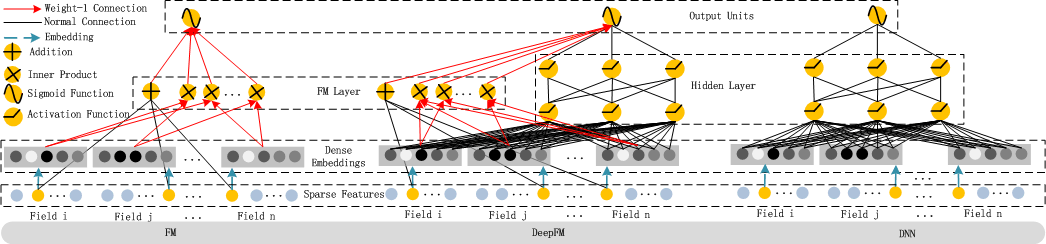
\includegraphics[width=0.96\textwidth]{img/architecture-wide.png}
%\caption{\footnotesize{The wide \& deep architecture of the proposed DeepFM. Note its wide (FM) component and deep component share the same input raw feature vector, and share the same embedding layer.}}\label{fig:architecture}
%\end{figure*}


We aim to learn both low- and high-order feature interactions. To this end, we propose a Factorization-Machine based neural network (DeepFM). As depicted in Figure~\ref{fig:architecture}\footnote{In all Figures of this paper, a \textbf{Normal Connection} in black refers to a connection with weight to be learned; a \textbf{Weight-1 Connection}, red arrow, is a connection with weight 1 by default; \textbf{Embedding}, blue dashed arrow, means a latent vector to be learned; \textbf{Addition} means adding all input together; \textbf{Product}, including \textbf{Inner-} and \textbf{Outer-Product}, means the output of this unit is the product of two input vector; \textbf{Sigmoid Function} is used as the output function in CTR prediction; \textbf{Activation Functions}, such as relu and tanh, are used for non-linearly transforming the signal.}, DeepFM consists of two components, \emph{FM component} and \emph{deep component}, that share  the same input. For feature $i$, a scalar $w_i$ is used to weigh its order-1 importance, a latent vector $V_i$ is used to measure its impact of interactions with other features. $V_i$ is fed in FM component to model order-2 feature interactions, and fed in deep component to model high-order feature interactions. All parameters, including $w_i$, $V_i$, and the network parameters ($W^{(l)}$, $b^{(l)}$ below) are trained jointly for the combined prediction model:
\begin{equation}
\hat{y}=sigmoid(y_{FM}+y_{DNN}),
\label{eq:FMNNCTR}
\end{equation}
where $\hat{y}\in (0,1)$ is the predicted CTR, $y_{FM}$ is the output of FM component, and $y_{DNN}$ is the output of deep component.
%\begin{equation}
%y_{DNN}=W^{|H|+1}\cdot a^{H}+b^{|H|+1}
%\label{eq:DNNoutput}
%\end{equation}
%where $|H|$ is the number of hidden layer.
%%\subsubsection{The FM Component}\label{section:App:model:fm}
%$y_{FM}$ is the output of FM component:
%\begin{equation}
%\centering
%y_{FM}=\left< w,x  \right> +\sum_{j_1=1}^{d}\sum_{j_2=j_1+1}^{d}\left< V_i,V_j  \right>  x_{j_1}\cdot x_{j_2}
%\label{eq:FM-model}
%\end{equation}
%$\hat{y}$ is the prediction, $x=[x_1,x_2,...,x_d]$ is a vector of $d$ features, $w=[w_1,w_2,...,w_d]$ are parameters to model the order-1 feature interactions, $V=[V_1,V_2,...,V_d]$ are parameters to model the order-2 feature interactions by inner product of the corresponding vectors, $V_i$ is the latent vector of feature $i$.
\subsubsection{FM Component}\label{section:App:model:fm}
\begin{figure}[ht]
\setlength{\abovecaptionskip}{0pt}%
\setlength{\belowcaptionskip}{-10pt}
\centering
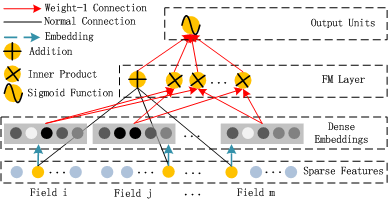
\includegraphics[width=0.42\textwidth]{img/architecture-fm.png}
\caption{\footnotesize{The architecture of FM. }}\label{fig:fm}
\end{figure}
The FM component is a factorization machine, which is proposed in \cite{fm} to learn feature interactions for recommendation. Besides a linear (order-1) interactions among features, FM models pairwise (order-2) feature interactions as inner product of respective feature latent vectors.
%Each latent vector is of length $k$, where k is a user-specified parameter.
It can capture order-2 feature interactions much more effectively than previous approaches especially when the dataset is sparse. In previous approaches, the parameter of an interaction of features $i$ and $j$ can be trained only when feature $i$ and feature $j$ both appear in the same data record. While in FM, it is measured via the inner product of their latent vectors $V_{i}$ and $V_{j}$. Thanks to this flexible design, FM can train latent vector $V_{i}$ ($V_{j}$) whenever $i$ (or $j$) appears in a data record. Therefore, feature interactions, which are never or rarely appeared in the training data, are better learnt by FM.

As Figure~\ref{fig:fm} shows, the output of FM is the summation of an \textbf{Addition} unit and a number of \textbf{Inner Product} units:
\begin{equation}
\centering
y_{FM}=\left< w,x  \right> +\sum_{j_1=1}^{d}\sum_{j_2=j_1+1}^{d}\left< V_i,V_j  \right>  x_{j_1}\cdot x_{j_2},
\label{eq:FM-model}
\end{equation}
where $w \in R^d$ and $V_i\in R^k$ ($k$ is given)\footnote{We omit a constant offset for simplicity.}. The Addition unit ($\left< w,x  \right>$) reflects the importance of order-1 features, and the Inner Product units represent the impact of order-2 feature interactions.
%\subsubsection{Logistic Regression (LR)}\label{section:App:back:lr}

%\begin{figure}[ht]
%\begin{center}
%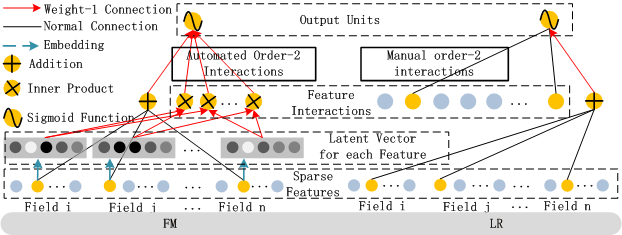
\includegraphics[width=0.48\textwidth]{img/LR+FM.png}
%\caption{\footnotesize{LR v.s. FM (The order-2 feature interactions are manually designed in LR, while they are automatically captured by the inner product of  the latent vector for each feature in FM.)}}\label{fig:lrfm}
%\end{center}
%\end{figure}
%
%As a simple yet effective and efficient approach, generalized linear models have shown great benefits in industrial CTR prediction. The model $w$ is obtained by solving a optimization problem:
%
%\begin{equation}
%\label{eq:LR}
%min_{w}=\frac{\lambda}{2}{\Vert w \Vert}_{2}^{2} + \sum_{i=1}^{n}log(1+exp(-y^i\phi_{LM}(w,x^i)))
%\end{equation}
%where $\lambda$ is the regularization parameter, and $\phi_{LM}(w,x^i)=w \cdot x^i$ is the prediction of the linear model.
%
%However, the widely-used logistic regression models are not be able to learn high-order feature interactions. Although manually designing order-2 feature interactions (namely, cross-product transformation) is a practical solution to enhance the logistic regression models (represented as LR-2), as presented in the right part of Figure~\ref{fig:lrfm}\footnote{In the figures of this paper, a \textbf{Normal Connection} in black refers to a connection with learnt weights; a \textbf{Weight-1 Connection}, represented by red arrow, is a connection with weight 1 and need not to be trained; \textbf{Embedding}, which is blue dashed arrow, means embedding for each feature; \textbf{Addition} means add all input together; \textbf{Product}, including \textbf{Inner-} and \textbf{Outer-Product}, means the output of this unit is the product of two input vector; \textbf{Sigmoid Function} is used as the output function in CTR prediction; \textbf{Activation Functions}, such as relu and tanh, are used for non-linearly transforming the signal.}, it cannot be generalized to the feature interactions that are never or rarely appeared in the training data.



\subsubsection{Deep Component}\label{section:App:model:dnn}
\begin{figure}[ht]
\setlength{\abovecaptionskip}{0pt}%
\setlength{\belowcaptionskip}{-10pt}
\centering
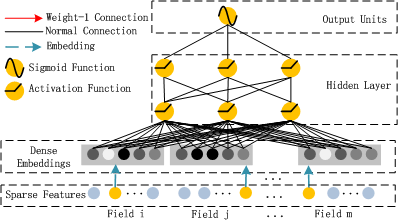
\includegraphics[width=0.42\textwidth]{img/architecture-dnn.png}
\caption{\footnotesize{The architecture of DNN.}}\label{fig:dnn}
\end{figure}
The deep component is a feed-forward neural network, which is used to learn high-order feature interactions. As shown in Figure~\ref{fig:dnn}, a data record (a vector) is fed into the neural network. Compared to neural networks with image~\cite{residual2016} or audio~\cite{audioBoulanger-LewandowskiBV13} data as input, which is purely continuous and dense, the input of CTR prediction is quite different, which requires a new network architecture design. Specifically, the raw feature input vector for CTR prediction is usually highly sparse\footnote{Only one entry is non-zero for each field vector.}, super high-dimensional\footnote{E.g., in an app store of billion users, the one field vector for user ID is already of billion dimensions.}, categorical-continuous-mixed, and grouped in fields (e.g., gender, location, age). This suggests an embedding layer to compress the input vector to a low-dimensional, dense real-value vector before further feeding into the first hidden layer, otherwise the network can be overwhelming to train.
\begin{figure}[ht]
\setlength{\abovecaptionskip}{0pt}%
\setlength{\belowcaptionskip}{-10pt}
\begin{center}
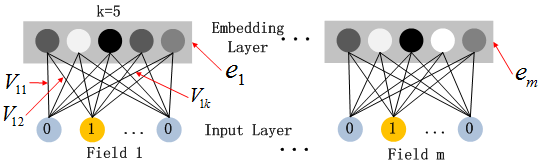
\includegraphics[width=0.40\textwidth]{img/embedding.png}
\caption{\footnotesize{The structure of the embedding layer}}\label{fig:embed}
\end{center}
\end{figure}
%$\mathbf{V^T_{start_{field_1}:end_{field_1}}\cdot x_{start_{field_1}:end_{field_1}}}$
%$\mathbf{e_{n}}$$\mathbf{e_{1}}$

Figure \ref{fig:embed} highlights the sub-network structure from the input layer to the embedding layer. We would like to point out the two interesting features of this network structure: 1) while the lengths of different input field vectors can be different, their embeddings are of the same size ($k$); 2) the latent feature vectors ($V$) in FM now server as network weights which are learned and used to compress the input field vectors to the embedding vectors. In \cite{fnn}, $V$ is pre-trained by FM and used as initialization. In this work, rather than using the latent feature vectors of FM to initialize the networks as in \cite{fnn}, we include the FM model as part of our overall learning architecture, in addition to the other DNN model. As such, we eliminate the need of pre-training by FM and instead jointly train the overall network in an end-to-end manner.
Denote the output of the embedding layer as:
\begin{equation}
\label{eq:embed}
a^{(0)}=[e_{1},e_{2},...,e_{m}],
 \end{equation}
where $e_{i}$ is the embedding of $i$-th field and $m$ is the number of fields. Then, $a^{(0)}$ is fed into the deep neural network, and the forward process is:


%each field, e.g., \textbf{city}, have multiple units, each of which presents a specific value of this field, e.g., \textbf{city=London}. Embedding each field to a latent vector independently results in reducing the embedding parameters from ${\mid a^{(0)}\mid}\cdot {\mid x \mid }$ to $k\cdot {\mid x \mid }$, where k is a small user-specified parameter to define the dimension of latent vectors. The output of the embedding layer is:
%\begin{equation}
%\label{eq:embed}
%a^{(0)}=[e_{field\_1},e_{field\_2},...,e_{|filed|}]
% \end{equation}
%where $a^{0}$ is fed into the first hidden layer, and $e_{field\_i}$ is the embedding of $i$-th field:
%\begin{equation}
%e_{field\_i} = V[{start_{field\_i}:end_{field\_i}}]\cdot x_{field\_i}
%\label{eq:embedconcat}
%\end{equation}
%where start$_{field\_i}$ and end$_{filed\_i}$ are starting and ending feature indexes of the $i$-th field.

\begin{equation}
\centering
\label{eq:h2h}
a^{(l+1)} = \sigma(W^{(l)}a^{(l)} + b^{(l)}),
\end{equation}
where $l$ is the layer depth and $\sigma$ is an activation function. $a^{(l)}$, $W^{(l)}$, $b^{(l)}$ are the output, model weight, and bias of the $l$-th layer. After that, a dense real-value feature vector is generated, which is finally fed into the sigmoid function for CTR prediction: $y_{DNN}=\sigma({W^{|H|+1}\cdot a^{H}+b^{|H|+1}})$, where $|H|$ is the number of hidden layers.
%\begin{equation}
%y_{DNN}=W^{|H|+1}\cdot a^{H}+b^{|H|+1}
%\label{eq:DNNoutput}
%\end{equation}



It is worth pointing out that FM component and deep component share the same feature embedding, which brings two important benefits: 1) it learns both low- and high-order feature interactions from raw features; 2) there is no need for expertise feature engineering of the input, as required in Wide \& Deep~\cite{wide-n-deep}.

\subsection{Relationship with the other Neural Networks}\label{section:App:rela}

Inspired by the enormous success of deep learning in various applications, several deep models for CTR prediction are developed recently. This section compares the proposed DeepFM with existing deep models for CTR prediction.

\begin{figure*}[ht]
\setlength{\abovecaptionskip}{0pt}%
\setlength{\belowcaptionskip}{-10pt}
\centering
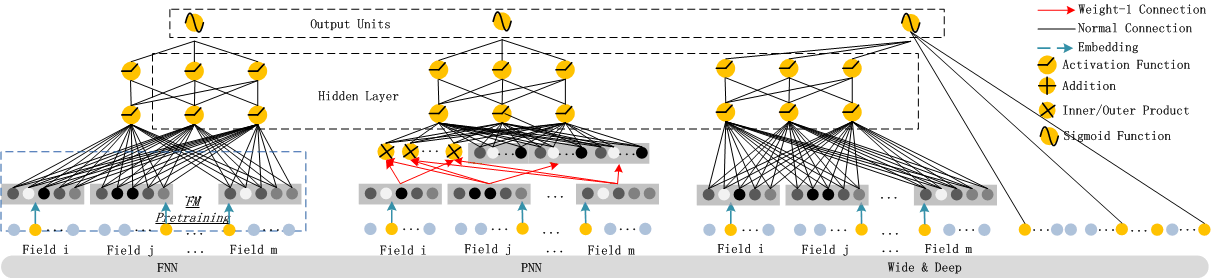
\includegraphics[width=0.92\textwidth]{img/Other-model.png}
\caption{\footnotesize{The architectures of existing deep models for CTR prediction: FNN, PNN, Wide \& Deep Model}}\label{fig:othermodel}
\end{figure*}

%\subsubsection{Factorization-machine supported Neural Network (FNN)}\label{section:App:rela:fnn}

\noindent\textbf{FNN:} As Figure~\ref{fig:othermodel} (left) shows, FNN is a FM-initialized feed-forward neural network~\cite{fnn}. The FM pre-training strategy results in two limitations: 1) the embedding parameters might be over affected by FM; 2) the efficiency is reduced by the overhead introduced by the pre-training stage. In addition, FNN captures only high-order feature interactions. In contrast, DeepFM needs no pre-training and learns both high- and low-order feature interactions.

%\subsubsection{Product-based Neural Network (PNN)}\label{section:App:rela:pnn}

\noindent\textbf{PNN:} For the purpose of capturing high-order feature interactions, PNN imposes a product layer between the embedding layer and the first hidden layer~\cite{pnn}. According to different types of product operation, there are three variants: IPNN, OPNN, and PNN$\ast$, where IPNN is based on inner product of vectors, OPNN is based on outer product, and PNN$\ast$ is based on both inner and outer products.

To make the computation more efficient, the authors proposed the approximated computations of both inner and outer products: 1) the inner product is approximately computed by eliminating some neurons; 2) the outer product is approximately computed by compressing $m$ $k$-dimensional feature vectors to one $k$-dimensional vector. However, we find that the outer product is less reliable than the inner product, since the approximated computation of outer product loses much information that makes the result unstable. Although inner product is more reliable, it still suffers from high computational complexity, because the output of the product layer is connected to all neurons of the first hidden layer. Different from PNN, the output of the product layer in DeepFM only connects to the final output layer (one neuron). Like FNN, all PNNs ignore low-order feature interactions.

%\subsubsection{Wide \& Deep}\label{section:App:rela:widedeep}

%\begin{figure}[ht]
%\centering
%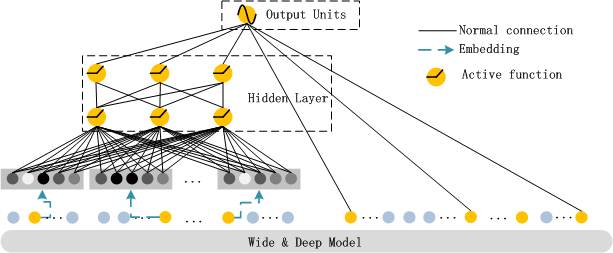
\includegraphics[width=0.48\textwidth]{img/wide-deep.png}
%\caption{{The Wide \& Deep model}}\label{fig:widedeep}
%\end{figure}

\noindent\textbf{Wide \& Deep:} Wide \& Deep (Figure~\ref{fig:othermodel} (right)) is proposed by Google to model low- and high-order feature interactions simultaneously. As shown in~\cite{wide-n-deep}, there is a need for expertise feature engineering on the input to the ``wide" part (for instance, cross-product of users' install apps and impression apps in app recommendation). In contrast, DeepFM needs no such expertise knowledge to handle the input by learning directly from the input raw features.

A straightforward extension to this model is replacing LR by FM  (we also evaluate this extension in Section~\ref{section:exp}). This extension is similar to DeepFM, but DeepFM shares the feature embedding between the FM and deep component. The sharing strategy of feature embedding influences (in back-propagate manner) the feature representation by both low- and high-order feature interactions, which models the representation more precisely.


\noindent\textbf{Summarizations:} To summarize, the relationship between DeepFM and the other deep models in four aspects is presented in Table~\ref{table:Modelcompare}. As can be seen, DeepFM is the only model that requires no pre-training and no feature engineering, and captures both low- and high-order feature interactions.

\begin{table}
\centering
\scriptsize
\caption{\footnotesize{Comparison of deep models for CTR prediction}}\label{table:Modelcompare}
\begin{tabular}{|c|c|c|c|c|}
\hline
 &  No& High-order  & Low-order  & No Feature \\
 &Pre-training     & Features     & Features    & Engineering \\ \hline
FNN & $\times$ & $\surd$  & $\times$ & $\surd$ \\ \hline
PNN & ${\surd}$ & ${\surd}$  & ${\times}$ & ${\surd}$ \\ \hline
Wide \& Deep & ${\surd}$   & ${\surd}$  & ${\surd}$  & ${\times}$\\ \hline
DeepFM & ${\surd}$ & ${\surd}$  & ${\surd}$  & ${\surd}$ \\ \hline
\end{tabular}
\end{table}
